\item \textbf{{[}ALVL/9597/2018/P2/Q6{]} }

Customers want to buy tickets for a diving championship that takes
place over three days. There are two sessions of diving each day. 

Customers use a ticket ordering website to buy their tickets.
\begin{center}
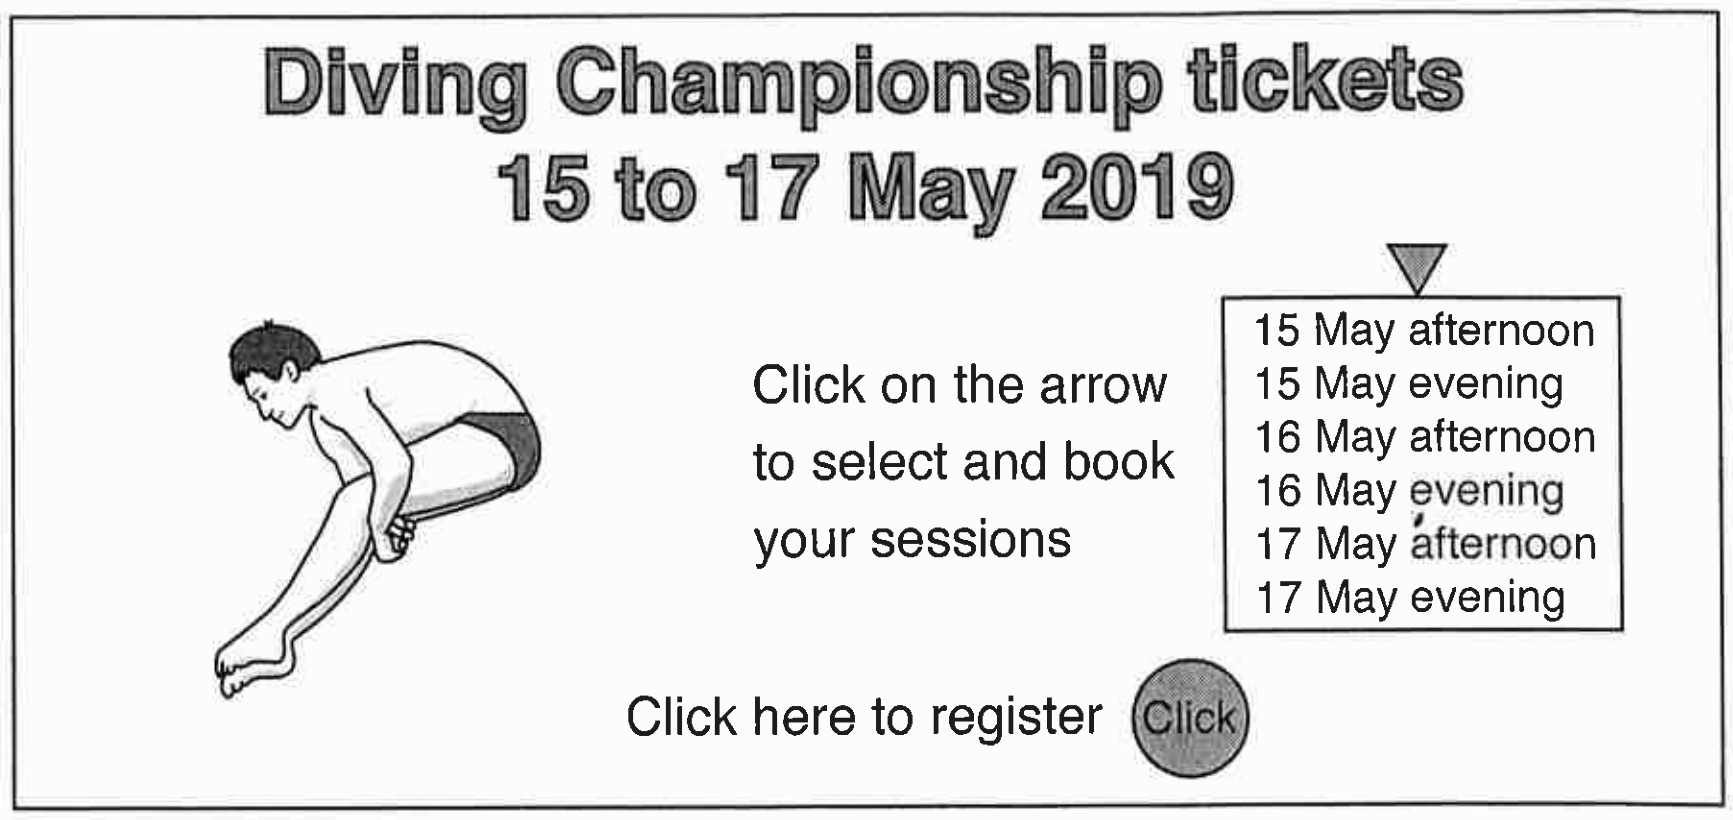
\includegraphics[width=0.5\paperwidth]{C:/Users/Admin/Desktop/Github/question_bank/LyX/static/img/9597-ALVL-2018-P2-Q6-1}
\par\end{center}
\begin{enumerate}
\item State the type of user interface that the ticket ordering website
uses. \hfill{}{[}1{]}
\item All ticket sales are stored on a database server in the following
tables: 

\texttt{CUSTOMER(}\texttt{\uline{CustomerID}}\texttt{, CustomerName,
Email, ContactNumber) }

\texttt{BOOKING(}\texttt{\uline{BookinoID}}\texttt{, BookingDate,
CustomerID) }

\texttt{SESSION(}\texttt{\uline{SessionID}}\texttt{, Date, Time,
SessionCost) }

\texttt{BOOKING\_SESSION(}\texttt{\uline{BookingID}}\texttt{, }\texttt{\uline{SessionID}}\texttt{,
Quantity)} 

\texttt{CustomerID} is the unique identifier in the \texttt{CUSTOMER}
table. 

\texttt{BookingID} is the unique identifier in the \texttt{BOOKING}
table. 

\texttt{SessionID} is the unique identifier in the \texttt{SESSION}
table. 
\begin{enumerate}
\item Draw an Entity-Relationship (E-R) diagram to represent this data model.
\hfill{}{[}4{]}
\item Name the fields that would be used to calculate the customer\textquoteright s
payment for a session. \hfill{}{[}2{]}
\end{enumerate}
\item Before customers can make an online ticket purchase, they have to
fill in a registration form. The details from this form are used to
complete the CUSTOMER table. 
\begin{center}
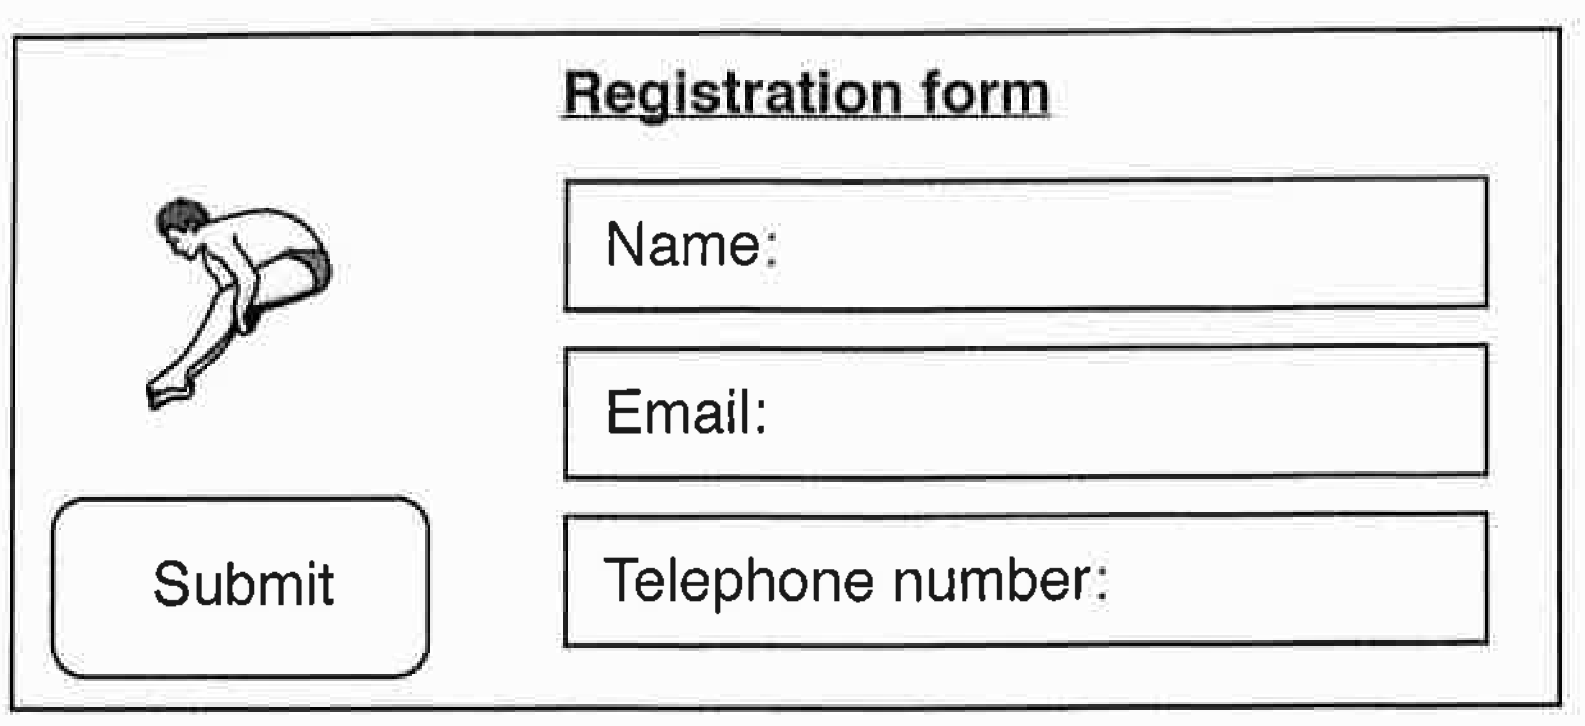
\includegraphics[width=0.5\paperwidth]{C:/Users/Admin/Desktop/Github/question_bank/LyX/static/img/9597-ALVL-2018-P2-Q6-2}
\par\end{center}

Explain how the web server will use server-side script to process
this form. \hfill{} {[}5{]}
\item The organisers of the championship store all the data for the event
using cloud storage. 

Describe\textbf{ three} economic benefits to the organisers of using
cloud-based storage. \hfill{}{[}3{]}
\end{enumerate}